\documentclass[conference]{IEEEtran}

% Single-file, Overleaf-ready source. All figures are drawn with TikZ/pgfplots.
% The block between the GENERATED DATA markers is written by
% docs/analysis/to_pgfplots.py from docs/analysis/results/*.csv; edit the data,
% not the block.
\usepackage{cite}
\usepackage{graphicx}
\usepackage{url}
\usepackage{booktabs}
\usepackage{tabularx}
\usepackage{array}
\usepackage{amsmath}
\usepackage{balance}
\usepackage{microtype}
\usepackage{xcolor}
\usepackage{tikz}
\usepackage{pgfplots}
\usepackage{pgfplotstable}
\pgfplotsset{compat=1.18}
\usetikzlibrary{arrows.meta,positioning,fit,calc,backgrounds}

\newcolumntype{Y}{>{\raggedright\arraybackslash}X}

% Validated categorical palette, reinforced with marker and dash for print.
\definecolor{seriesA}{HTML}{2A78D6}
\definecolor{seriesB}{HTML}{EB6834}
\definecolor{seriesC}{HTML}{1BAF7A}
\definecolor{statusNormal}{HTML}{E4E4E0}
\definecolor{statusWarning}{HTML}{FAB219}
\definecolor{statusFailed}{HTML}{D03B3B}
\definecolor{ink}{HTML}{52514E}
\pgfplotsset{
  paperaxis/.style={
    font=\footnotesize, tick label style={font=\scriptsize},
    label style={font=\scriptsize}, title style={font=\footnotesize, yshift=-3pt},
    legend style={font=\scriptsize, draw=none, fill=none},
    axis line style={ink}, tick style={ink},
    grid style={black!12}, axis lines*=left},
}
\tikzset{
  built/.style={draw, thick, rounded corners=1.5pt, align=center, font=\scriptsize, inner sep=3pt, fill=seriesA!9},
  planned/.style={draw, dashed, rounded corners=1.5pt, align=center, font=\scriptsize, inner sep=3pt},
  idle/.style={draw, dotted, rounded corners=1.5pt, align=center, font=\scriptsize, inner sep=3pt},
  tier/.style={font=\scriptsize\bfseries, text=ink},
  flow/.style={-{Latex[length=4pt]}, thick},
  plan/.style={-{Latex[length=4pt]}, dashed},
}

%%% BEGIN GENERATED DATA
\pgfplotstableread{
label pressure flow
{Tank} 40.0 0.0
{Pipe A} 38.0 38.0
{Valve} 38.0 19.0
{Pipe B} 34.0 34.0
{Tap} 38.0 38.0
}\tableProfile
\newcommand{\pressTank}{40}
\newcommand{\flowTank}{0}
\newcommand{\pressPipeA}{38}
\newcommand{\flowPipeA}{38}
\newcommand{\pressValve}{38}
\newcommand{\flowValve}{19}
\newcommand{\pressPipeB}{34}
\newcommand{\flowPipeB}{34}
\newcommand{\pressTap}{38}
\newcommand{\flowTap}{38}
\newcommand{\onsetWarnTap}{100.4}
\newcommand{\onsetFailTap}{122.1}
\newcommand{\onsetWarnPipeB}{63.5}
\newcommand{\onsetFailPipeB}{76.1}
\newcommand{\onsetWarnValve}{125.0}
\newcommand{\onsetFailValve}{152.1}
\newcommand{\onsetWarnPipeA}{59.5}
\newcommand{\onsetFailPipeA}{72.1}
\newcommand{\onsetWarnTank}{164.1}
\newcommand{\onsetFailTank}{200.1}
\pgfplotstableread{
label normal warning failed
{Tap} 100.4 21.7 177.9
{Pipe B} 63.5 12.6 223.9
{Valve} 125.0 27.1 147.9
{Pipe A} 59.5 12.6 227.9
{Tank} 164.1 36.0 99.9
}\tableBands
\newcommand{\closedPipeB}{0}
\newcommand{\closedTap}{0}
\pgfplotstableread{
n median
5 0.0384
10 0.0707
25 0.1766
50 0.3766
100 0.9562
250 3.8733
500 14.5105
1000 57.7881
2000 222.4982
}\tableScale
\newcommand{\scaleFive}{0.038}
\newcommand{\scaleHundred}{0.96}
\newcommand{\scaleOneK}{57.8}
\newcommand{\scaleTwoK}{222}
\newcommand{\scaleDoubling}{3.9}
\newcommand{\scaleSlope}{1.84}
\newcommand{\rttN}{1{,}000}
\newcommand{\rttPfifty}{7.5}
\newcommand{\rttPninetyfive}{8.5}
\newcommand{\rttPninetynine}{9.2}
\newcommand{\simBytes}{3{,}572}
\pgfplotstableread{
clients p50 err
1 4.888 0.744
2 4.877 0.718
5 5.045 0.934
10 5.148 0.857
25 5.654 1.140
50 6.371 1.822
}\tableFanEvent
\newcommand{\fanEventPfiftyA}{4.9}
\newcommand{\fanEventPninetyfiveA}{5.6}
\newcommand{\fanEventMaxA}{8}
\newcommand{\fanEventLastA}{5.6}
\newcommand{\fanEventPfiftyB}{4.9}
\newcommand{\fanEventPninetyfiveB}{5.6}
\newcommand{\fanEventMaxB}{20}
\newcommand{\fanEventLastB}{5.6}
\newcommand{\fanEventPfiftyC}{5.0}
\newcommand{\fanEventPninetyfiveC}{6.0}
\newcommand{\fanEventMaxC}{13}
\newcommand{\fanEventLastC}{6.1}
\newcommand{\fanEventPfiftyD}{5.1}
\newcommand{\fanEventPninetyfiveD}{6.0}
\newcommand{\fanEventMaxD}{22}
\newcommand{\fanEventLastD}{6.3}
\newcommand{\fanEventPfiftyE}{5.7}
\newcommand{\fanEventPninetyfiveE}{6.8}
\newcommand{\fanEventMaxE}{14}
\newcommand{\fanEventLastE}{7.4}
\newcommand{\fanEventPfiftyF}{6.4}
\newcommand{\fanEventPninetyfiveF}{8.2}
\newcommand{\fanEventMaxF}{14}
\newcommand{\fanEventLastF}{9.4}
\newcommand{\fanEventBytes}{767}
\pgfplotstableread{
clients p50 err
1 10.651 1.434
2 13.416 1.346
5 22.493 2.660
10 36.866 17.164
25 83.032 35.833
}\tableFanGet
\newcommand{\fanGetPfiftyA}{10.7}
\newcommand{\fanGetPninetyfiveA}{12.1}
\newcommand{\fanGetMaxA}{32}
\newcommand{\fanGetLastA}{12.1}
\newcommand{\fanGetPfiftyB}{13.4}
\newcommand{\fanGetPninetyfiveB}{14.8}
\newcommand{\fanGetMaxB}{19}
\newcommand{\fanGetLastB}{14.9}
\newcommand{\fanGetPfiftyC}{22.5}
\newcommand{\fanGetPninetyfiveC}{25.2}
\newcommand{\fanGetMaxC}{56}
\newcommand{\fanGetLastC}{25.8}
\newcommand{\fanGetPfiftyD}{36.9}
\newcommand{\fanGetPninetyfiveD}{54.0}
\newcommand{\fanGetMaxD}{93}
\newcommand{\fanGetLastD}{57.2}
\newcommand{\fanGetPfiftyE}{83.0}
\newcommand{\fanGetPninetyfiveE}{118.9}
\newcommand{\fanGetMaxE}{162}
\newcommand{\fanGetLastE}{129.6}
\newcommand{\fanGetBytes}{767}
\pgfplotstableread{
clients p50 err
nan nan nan
}\tableFanSim
\newcommand{\fanSamples}{122{,}400}
\newcommand{\fanDelivered}{134{,}640}
\newcommand{\fanTimeouts}{0}
\newcommand{\lostTrials}{500}
\newcommand{\lostConc}{500}
\newcommand{\lostConcOpen}{267}
\newcommand{\lostConcPos}{233}
\newcommand{\lostSeq}{500}
\newcommand{\lostSeqOpen}{500}
\newcommand{\lostSeqPos}{0}
\newcommand{\lostFresh}{0}
\newcommand{\lostFreshOpen}{0}
\newcommand{\lostFreshPos}{0}
\newcommand{\awaySent}{400}
\newcommand{\awayReplayed}{0}
\newcommand{\awayControl}{400}
\newcommand{\awayStale}{20}
\newcommand{\awayTrials}{20}
\pgfplotstableread{
n idle sim simlow
nan nan nan nan
}\tableFrames
\newcommand{\framesMissing}{1}
\newcommand{\bundleGzKB}{\textbf{[pending]}}
\newcommand{\bundleKB}{\textbf{[pending]}}
\newcommand{\churnErrors}{\textbf{[pending]}}
\newcommand{\churnJoins}{\textbf{[pending]}}
\newcommand{\churnSeconds}{\textbf{[pending]}}
\newcommand{\churnUpdates}{\textbf{[pending]}}
\newcommand{\fanGetPfiftyF}{\textbf{[pending]}}
\newcommand{\fanSimBytes}{\textbf{[pending]}}
\newcommand{\fanSimPfiftyF}{\textbf{[pending]}}
\newcommand{\fpsIdleFive}{\textbf{[pending]}}
\newcommand{\fpsIdleTwoHundred}{\textbf{[pending]}}
\newcommand{\fpsLowTwoHundred}{\textbf{[pending]}}
\newcommand{\fpsSimFive}{\textbf{[pending]}}
\newcommand{\fpsSimTwoHundred}{\textbf{[pending]}}
\newcommand{\gpuName}{\textbf{[pending]}}
%%% END GENERATED DATA

\title{SpatialTwin-IoT: A Bidirectional Mixed-Reality and Web3D Digital-Twin Framework for Smart Fluid Systems and Interactive Industrial Assemblies}

\author{\IEEEauthorblockN{Gopal Krishna J S, M Aaryamann Prabhu, Dr. Andhe Dharani}
\IEEEauthorblockA{Department of Master of Computer Applications\\
RV College of Engineering\textsuperscript{\textregistered}, Bengaluru, India}}

\begin{document}
\maketitle

\begin{abstract}
Cheap sensors have made it practical to instrument plumbing networks and small fluid assemblies, yet browser tools and mixed-reality (MR) viewers rarely share one authoritative model of the same assembly. SpatialTwin-IoT is our framework for closing that gap. It joins an ESP32 telemetry tier, a FastAPI synchronization service, a React Three Fiber configurator, and MR clients for HoloLens 2 and XREAL One Pro around a device-independent component-and-port graph. The editor, simulator, and event service run today as PipeLab; the ESP32 and MR tiers are still planned, and we separate the two throughout. We measured the running baseline on one laptop over loopback. A simulation request took a median of \rttPfifty~ms, and with 50 subscribed clients a peer saw an update in \fanEventPfiftyF~ms, or \fanGetPfiftyF~ms once it had fetched the new state as the browser does. The same tests exposed the faults the proposed design targets: an edit made from a stale snapshot lost data in all \lostTrials{} trials, no event sent during a disconnection was recovered, and simulator runtime grew nearly quadratically with network size. The 100~ms sensor-to-client target remains untested because no sensor is connected yet.
\end{abstract}

\begin{IEEEkeywords}
Augmented reality, digital twin, mixed reality, Internet of Things, spatial registration, Web3D.
\end{IEEEkeywords}

\section{Introduction}
When a fault spreads through the valves, pipes, and outlets of a fluid system, finding where it started can take a long time. Microcontrollers such as the ESP32 can now collect flow and pressure data from these assemblies at low cost, and headsets and browser-based 3D renderers offer new ways to look at that data in place. Displaying the data is the easy part. The sensors, the browser, and the headset also have to agree on which components exist and what state each one is in. If a valve is closed in the browser, the MR view has to show it closed. If each viewer keeps its own copy of the state, an operator can end up inspecting a model that no longer matches the system.

A useful twin therefore needs a single source of truth, defined update rules, and measured limits on how quickly a change reaches everyone. Earlier work covers MR interfaces for twins, links between simulated and physical systems, and browser-delivered twin platforms \cite{tu2021crane,tu2023twinxr,hao2024roadheader,kaarlela2023robotics,tran2025usd,hlayel2025latency,liang2020bridge,li2025platform,lei2022labs}. Less attention has gone to the combination considered here, where an ESP32-class sensor, an MR viewer, and a browser configurator all work from one model that records where each update came from and in what order.

We build SpatialTwin-IoT on PipeLab, our browser-based plumbing-network editor. This paper makes four contributions:
\begin{enumerate}
  \item A device-independent plumbing-network model that ties telemetry, MR, and Web3D clients together through stable component and port identifiers, already implemented in PipeLab.
  \item A bidirectional synchronization design with explicit origin, timestamp, revision, and field-ownership rules. It is not yet implemented, and we show by experiment why the baseline needs it.
  \item A reproducible evaluation of the baseline covering simulator behavior, simulator scaling, fan-out latency, state convergence, and browser rendering. Every plot comes from a script published with the source.
  \item A portability boundary between what all clients share and what stays device-specific, including the real tracking differences between HoloLens 2 and XREAL One Pro.
\end{enumerate}

ESP32 integration, live telemetry, the MR clients, spatial anchors, and user studies do not exist yet. Where we discuss them we are describing a design, and we report no results for them.

\section{Related Work}
\subsection{Mixed-Reality Digital Twins}
Tu \emph{et al.} built an MR interface for a digital-twin overhead crane \cite{tu2021crane}, then generalized the idea in TwinXR, which drives industrial XR applications from ontology-based twin descriptions \cite{tu2023twinxr}. Hao \emph{et al.} used HoloLens and socket communication to monitor a coal-mine roadheader \cite{hao2024roadheader}. Kaarlela \emph{et al.} applied XR twins to robot training \cite{kaarlela2023robotics}, and Tran \emph{et al.} delivered real-time, multi-user AR over USD-based twins \cite{tran2025usd}. Valladares-Poncela \emph{et al.} added on-device speech recognition to an industrial MR application \cite{valladares2025speech}, which is why we treat speech as optional and leave it out of the first version. These systems focus on visualization and interaction. None sets out a shared state model spanning low-cost sensing, MR, and Web3D together.

\subsection{Synchronization and Web3D Delivery}
Liang \emph{et al.} built a bidirectional bridge that keeps digital-twin simulations and physical construction robots in step \cite{liang2020bridge}. Hlayel \emph{et al.} analyzed the latency of WebSocket and industrial protocols for twin integration \cite{hlayel2025latency}. Amirkhanov \emph{et al.} compared HTTP and MQTT from an ESP32 and reported mean latencies of roughly 290 to 340~ms \cite{amirkhanov2025evaluating}, a useful warning that our 100~ms target is not a given. On the web side, Li and Hong presented an open, web-based platform that merges building sensor data with simulation models \cite{li2025platform}, Lei \emph{et al.} surveyed methods for web-based twin laboratories \cite{lei2022labs}, Leggett \emph{et al.} delivered a tunnel twin through Web3D \cite{leggett2025permafrost}, and Lee and Yoo examined XR collaboration in physical work \cite{lee2021collaboration}. This work shaped our decision to start from one FastAPI service and a WebSocket channel, and to add a broker only when measurements call for it.

\subsection{Research Gap}
In the work we reviewed, we did not find these four elements brought together: an ESP32-class edge tier; a state model that separates telemetry-owned fields from user-owned fields; synchronized MR and Web3D clients; and an evaluation that reports what each headset can actually track. SpatialTwin-IoT targets that combination. So far we can back the shared model and the Web3D side with running code and data.

\section{System Requirements and Architecture}
\subsection{Use Case and Principles}
Our reference assembly is a small physical rig with a tank, a pipe run, a valve, a flow sensor on an ESP32, and an outlet. Operators perform four tasks: find a named valve and its upstream and downstream neighbors; find a reported failure, its cause, and the outlet it affects; change a valve and confirm that a second client shows the change; and realign the model after losing tracking, on devices where that task is possible. The tasks are defined on assembly state, not on any display, so they can be compared across clients.

Four principles guide the design. The service holds the \emph{one authoritative state}: clients load a snapshot, subscribe to events, and submit edits through the API. Every update carries an \emph{explicit origin and timestamp}, so ordering and delay can be reconstructed from logs. \emph{Field ownership} divides the data: flow rate, pulse count, and sensor-quality flags belong to telemetry, while valve setpoints, placement, and configuration belong to users, and neither side may overwrite the other. Finally, the \emph{model is shared while interaction is device-specific}: identifiers, graph structure, units, and event envelopes are common, whereas tracking, anchors, input, and rendering belong to each client. The first and last principles hold in PipeLab today. Origin tracking and ownership do not (Table~\ref{tab:status}).

\subsection{Three-Tier Architecture}
Fig.~\ref{fig:architecture} shows the architecture, with solid boxes for what runs today and dashed boxes for what is planned. The edge tier will publish timestamped, sequence-numbered measurements. The synchronization tier validates messages, updates the authoritative state, persists it, and broadcasts events. The client tier holds the browser configurator and, later, the MR viewers.

\begin{figure}[t]
\centering
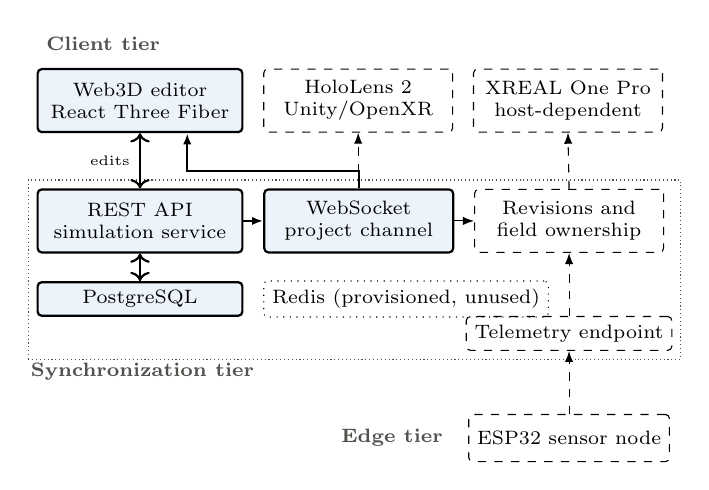
\begin{tikzpicture}[node distance=3mm and 2.5mm]
  \node[tier] (t3) {Client tier};
  \node[built, below=1mm of t3.south west, anchor=north west, minimum width=26mm, minimum height=8mm] (web) {Web3D editor\\React Three Fiber};
  \node[planned, right=of web, minimum width=24mm, minimum height=8mm] (holo) {HoloLens 2\\Unity/OpenXR};
  \node[planned, right=of holo, minimum width=24mm, minimum height=8mm] (xreal) {XREAL One Pro\\host-dependent};

  \node[built, below=7mm of web, minimum width=26mm, minimum height=8mm] (rest) {REST API\\simulation service};
  \node[built, right=of rest, minimum width=24mm, minimum height=8mm] (ws) {WebSocket\\project channel};
  \node[planned, right=of ws, minimum width=24mm, minimum height=8mm] (rev) {Revisions and\\field ownership};

  \node[built, below=3.5mm of rest, minimum width=26mm] (db) {PostgreSQL};
  \node[idle, right=of db, minimum width=24mm] (redis) {Redis (provisioned, unused)};
  \node[planned, below=8mm of rev, minimum width=24mm] (tele) {Telemetry endpoint};

  \node[planned, below=8mm of tele, minimum width=24mm, minimum height=6mm] (esp) {ESP32 sensor node};
  \node[tier, anchor=east] at ($(esp.west)+(-2mm,0)$) {Edge tier};

  \begin{scope}[on background layer]
    \node[draw=ink, densely dotted, inner sep=3pt, fit=(rest)(ws)(rev)(db)(redis)(tele), label={[tier, anchor=north west, inner sep=1pt]south west:Synchronization tier}] (sync) {};
  \end{scope}

  \draw[flow, <->] (web.south) -- node[left, font=\tiny] {edits} (rest.north);
  \draw[flow] (ws.north) -- ++(0,2.2mm) -| ([xshift=6mm]web.south);
  \draw[plan] (ws.north) -- ++(0,2.2mm) -| (holo.south);
  \draw[plan] (rev.north) -- (xreal.south);
  \draw[flow] (rest) -- (ws);
  \draw[plan] (ws) -- (rev);
  \draw[flow, <->] (rest) -- (db);
  \draw[plan] (tele) -- (rev);
  \draw[plan] (esp) -- (tele);
\end{tikzpicture}
\caption{Three-tier architecture. Shaded solid boxes run in the repository today, dashed boxes are planned, and the dotted Redis container is provisioned but unused.}
\label{fig:architecture}
\end{figure}

\subsection{Coordinates, Ownership, and Conflicts}
Geometry is stored in component-local coordinates and mapped to project coordinates by each component's position and rotation. The planned MR path adds a separate transform or anchor reference from project coordinates to the physical rig, so a headset's temporary origin never enters the engineering model. QR-based alignment is a candidate calibration method. We make no accuracy claim until error has been measured against a surveyed reference.

In the planned update path, sensor messages may write only telemetry-owned fields and clients may write only user-owned fields. Each update carries a revision, the service rejects stale ones, and a client that falls behind receives a divergence event. These rules are design, not code. Section~\ref{sec:convergence} measures what happens without them.

\section{Implementation}
\subsection{The PipeLab Baseline}
The front end is about 3,000 lines of TypeScript. A React Three Fiber scene renders a domain graph, which holds no Three.js state, through a Zustand store. Each component has a stable identifier, one of six types (tank, pipe, elbow, valve, tap, custom), a material, a pressure rating, and named ports with a local position, direction, and diameter. Connections reference component and port identifiers, so hydraulic connectivity never depends on visual proximity. Fig.~\ref{fig:graph} shows the seed network as this graph.

\begin{figure}[t]
\centering
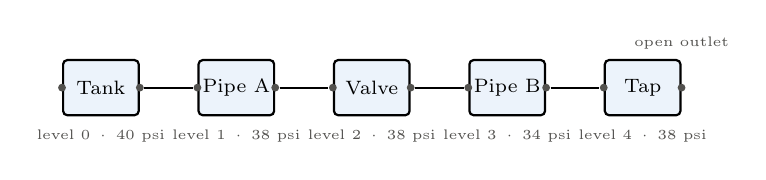
\begin{tikzpicture}[
  part/.style={draw, thick, rounded corners=1.5pt, minimum width=9.6mm, minimum height=7mm, font=\scriptsize, fill=seriesA!9, inner sep=1pt, align=center},
  portdot/.style={circle, fill=ink, inner sep=1pt},
  lbl/.style={font=\tiny, text=ink}]
  \foreach \i/\n/\l in {0/tank/Tank, 1/pa/Pipe A, 2/val/Valve, 3/pb/Pipe B, 4/tap/Tap}{
    \node[part] (\n) at (\i*1.72,0) {\l};
    \node[portdot] (\n R) at (\n.east) {};
    \node[portdot] (\n L) at (\n.west) {};
  }
  \foreach \a/\b in {tank/pa, pa/val, val/pb, pb/tap}{ \draw[thick] (\a R) -- (\b L); }
  \node[lbl, anchor=south] at (tap.north east) {open outlet};
  \foreach \n/\lev/\p in {tank/0/\pressTank, pa/1/\pressPipeA, val/2/\pressValve, pb/3/\pressPipeB, tap/4/\pressTap}{
    \node[lbl, below=0.5mm of \n] {level \lev{} \,$\cdot$\, \p{} psi};
  }
\end{tikzpicture}
\caption{The seed network as a component-and-port graph. Dots are named ports. Labels give the breadth-first level and the simulated pressure at a 40~psi source.}
\label{fig:graph}
\end{figure}

The back end is a FastAPI service with 16 HTTP routes and a single WebSocket route, about 370 lines of Python. Docker Compose runs it with PostgreSQL, and SQLite serves as a fallback for direct runs. Clients load a project, send each edit through REST, and subscribe to \texttt{/ws/projects/\{id\}}. Events use a \{\texttt{version}, \texttt{type}, \texttt{project\_id}, \texttt{payload}\} envelope. The editor also offers snap-to-port placement within a 1.5-unit radius, breadth-first auto-alignment, and import of GLB, OBJ, and FBX meshes. Imported meshes live in one browser's IndexedDB: the asset identifier syncs, but the bytes do not, so a second client cannot yet draw them. Table~\ref{tab:status} maps the design against the repository.

\begin{table}[t]
\caption{Design Elements Against the Repository}
\label{tab:status}
\centering
\footnotesize
\begin{tabularx}{\columnwidth}{@{}p{0.37\columnwidth}Yl@{}}
\toprule
\textbf{Element} & \textbf{In the code today} & \textbf{Status}\\
\midrule
Component-port graph & Stable IDs, typed ports & Built\\
Event channel & Four-field envelope, version fixed at 1 & Built\\
Persistence & PostgreSQL, SQLite fallback & Built\\
Simulator & Graph heuristic, no solver & Demo only\\
Mesh import & Local to one browser & Partial\\
PBR materials & Standard material, no toggle & Partial\\
Broker fan-out & Redis runs, nothing calls it & Unused\\
Revision, origin, sequence & Absent from the envelope & Planned\\
Field ownership & \texttt{PUT} replaces the whole row & Planned\\
Snapshot and replay & No reconnect logic & Planned\\
Authentication & None; CORS open to all & Planned\\
Draco, exploded view, audio & Absent & Planned\\
ESP32, telemetry route & Absent & Planned\\
MR clients, anchors & Absent & Planned\\
\bottomrule
\end{tabularx}
\end{table}

\subsection{Simulator}
All results come from the API; the browser does not compute them. The service runs a breadth-first search from the tank to assign each reachable component $i$ a level $\ell_i$, stopping at closed valves and taps. It then computes
\begin{equation}
p_i = \max\bigl(0,\; P_s - \ell_i\, d(\tau_i)\bigr), \qquad
q_i = \frac{o_i\, p_i}{\max(1, r_i)},
\label{eq:sim}
\end{equation}
where $P_s$ is the source pressure, $d(\tau_i)$ is a fixed drop of 2, 1, or 0.5 for a pipe, a valve, or anything else, $o_i$ is the valve opening, and $r_i$ is the flow resistance. Health and remaining life follow from age, fluid type, and pressure ratio. Unconnected ports on pressurized parts become leaks, parts at or above their rating become breaks, and the first failed part is named as the root cause.

This model drives the visualization and the diagnostics demo. It is a heuristic and not a hydraulic solver. Section~\ref{sec:simresults} shows how far it departs from physical behavior.

\subsection{Update Path}
Fig.~\ref{fig:sequence} traces one edit. The writer sends the full component in a \texttt{PUT}. The service replaces the row, commits, and sends \texttt{component\_updated} to each subscriber in turn. On any event other than a simulation result, the browser discards the payload and fetches the whole project again. That keeps clients simple and consistent with the database, at the price of one extra request per client per event. The planned path adds the steps shown dashed.

\begin{figure}[t]
\centering
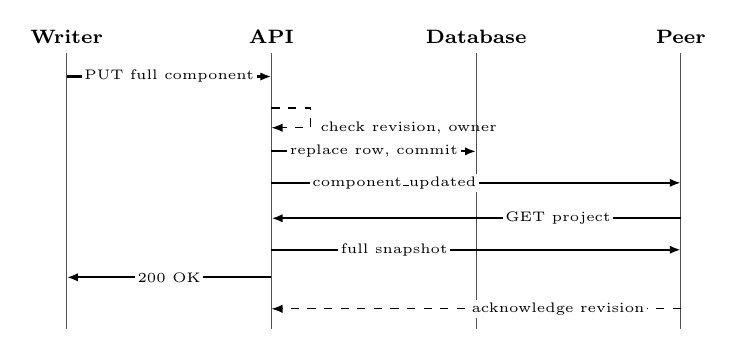
\begin{tikzpicture}[
  actor/.style={font=\scriptsize\bfseries, inner sep=1pt},
  msg/.style={font=\tiny, fill=white, inner sep=1pt},
  lane/.style={ink, thin}, x=1mm, y=1mm]
  \def\ya{0}\def\yb{26}\def\yc{52}\def\yd{78}
  \node[actor] at (\ya,0) {Writer};
  \node[actor] at (\yb,0) {API};
  \node[actor] at (\yc,0) {Database};
  \node[actor] at (\yd,0) {Peer};
  \foreach \x in {\ya,\yb,\yc,\yd}{ \draw[lane] (\x,-2) -- (\x,-37); }
  \draw[flow] (\ya,-5) -- node[msg] {PUT full component} (\yb,-5);
  \draw[plan] (\yb,-9) -- ++(5,0) -- ++(0,-2.5) node[right, font=\tiny] {check revision, owner} -- ++(-5,0);
  \draw[flow] (\yb,-14.5) -- node[msg] {replace row, commit} (\yc,-14.5);
  \draw[flow] (\yb,-18.5) -- node[msg, pos=.3] {component\_updated} (\yd,-18.5);
  \draw[flow] (\yd,-23) -- node[msg, pos=.3] {GET project} (\yb,-23);
  \draw[flow] (\yb,-27) -- node[msg, pos=.3] {full snapshot} (\yd,-27);
  \draw[flow] (\yb,-30.5) -- node[msg] {200 OK} (\ya,-30.5);
  \draw[plan] (\yd,-34.5) -- node[msg, pos=.3] {acknowledge revision} (\yb,-34.5);
\end{tikzpicture}
\caption{One edit as implemented (solid), with the planned revision check and acknowledgement (dashed). The service sends to peers before it answers the writer.}
\label{fig:sequence}
\end{figure}

\subsection{Planned Edge Tier}
The ESP32 will count flow-sensor pulses with an interrupt routine and read analog values, then send device and sensor identifiers, a capture time, a sequence number, units, and quality flags. Bounded queues will stop a slow network from blocking acquisition. We do not assume that every pulse is counted, so bench tests will compare counts with a controlled pulse source. Payloads stay in JSON until measurements say otherwise.

\subsection{Planned MR Pathways}
HoloLens 2 will use a Unity and OpenXR client with hand and gaze input and native spatial anchors, subject to checks on the real device. XREAL One Pro needs more care. Its built-in modes offer 3DoF rotational tracking, which does not by itself give world-locked placement, spatial mapping, or persistent anchors. Unless a supported host-tracked setup provides these, the XREAL path will be screen-anchored. Table~\ref{tab:tracking} records the difference, and we treat it as a finding about portability and not as a gap to paper over.

\begin{table}[t]
\caption{Tracking and Input Across the Client Pathways}
\label{tab:tracking}
\centering
\footnotesize
\begin{tabularx}{\columnwidth}{@{}p{0.27\columnwidth}p{0.24\columnwidth}Y@{}}
\toprule
\textbf{Client} & \textbf{Input} & \textbf{Coordinates}\\
\midrule
HoloLens 2 (6DoF) & Hand, gaze & World-locked anchors, to be verified\\
XREAL One Pro (3DoF) & Host-dependent & Screen-anchored or host-tracked\\
Web3D (none) & Mouse, keyboard & Project coordinates\\
\bottomrule
\end{tabularx}
\end{table}

\section{Evaluation Method}
\label{sec:method}
\subsection{Research Questions}
We organize the evaluation around five questions. \textbf{RQ1:} Do sensor updates and client edits converge to one authoritative state, in normal use and after reconnects? \textbf{RQ2:} What latency and delivery does the system show at given rates, networks, and client counts? \textbf{RQ3:} Which tasks are feasible with the tracking and input that HoloLens 2 and XREAL One Pro actually offer? \textbf{RQ4:} What frame rate and loading behavior does the browser configurator achieve on named hardware? \textbf{RQ5:} Which constraints limit use of the framework across clients?

Without sensors or headsets, we can address RQ1 and RQ2 in part, RQ4 directly, and RQ3 not at all. Our predefined targets are 100~ms from sensor capture to visible client update, and 60 frames per second (FPS) for Web3D rendering.

\subsection{Test Bed}
All experiments ran on one laptop with an Intel Core i5-10300H, 16~GB of RAM, and \gpuName{}, under Arch-based Linux. The stack was the repository's own Compose deployment: one uvicorn worker on Python 3.12, with PostgreSQL 16. Client processes ran on the same machine, so traffic used loopback through the container's published port. Each latency was taken on one monotonic clock in the test client, which removes clock synchronization as a source of error. The server was not instrumented, and the application code was not changed.

\subsection{Experiments and Boundaries}
\emph{E1} runs the simulator on the seed network across its accepted range of 0 to 300~psi. \emph{E2} times it on series chains of 5 to 2,000 components. \emph{E3} sends \rttN{} simulation requests. \emph{E4} measures action-to-peer latency for 1 to 50 subscribers, with 300 updates in each of three runs after a warm-up of 30. Each update waits for the previous one, so the service is never overloaded. E4 has three series: time to the \texttt{component\_updated} event; time to the event plus the project fetch that the browser performs; and time to a \texttt{simulation\_completed} event. Error bars run from the median to the 95th percentile. \emph{E5} has two clients edit different fields of one component in \lostTrials{} trials per arm, then counts events recovered after a disconnection. \emph{E6} opens and closes sockets during broadcasts. \emph{E7} measures the production bundle and, in a real Chromium window, frame intervals for scenes of 5 to 200 components.

These boundaries matter. E3 and E4 cover only the path from a client through the service to another client, so they are \emph{not} a test of the 100~ms target. That target also includes acquisition, the wireless link, and rendering. They show how much of the budget the service itself consumes.

\subsection{Planned Hardware and User Studies}
Once the edge tier exists, a reference flow meter or pulse source will validate the ESP32 readings, and clocks will be synchronized with a measured offset. Registration will be measured against a surveyed fixture. A small feasibility study, covering task completion, System Usability Scale, and NASA-TLX, may follow if ethics approval and hardware allow. If only one MR configuration proves practical, we will report feasibility and make no cross-device claims.

\section{Results}
\label{sec:results}
\subsection{Simulator Behavior}
\label{sec:simresults}
Fig.~\ref{fig:sim}(a) and (b) show the seed network at 40~psi. Pressure is not monotonic along the path: it reads \pressPipeB{}~psi at Pipe~B and then rises to \pressTap{}~psi at the tap downstream. Equation~\eqref{eq:sim} explains why, since each component's drop is its own type's value multiplied by its level, with no accumulation along the path. Flow is not conserved either. In a series run with no branches, it ranges from \flowValve{} at the valve to \flowTap{} at the tap. The stored \texttt{pressure\_loss} field is never read, and the seed's displayed starting pressures disagree with the simulator's.

The status logic behaves as designed. Fig.~\ref{fig:sim}(c) shows that Pipe~A reaches warning at \onsetWarnPipeA{}~psi and failure at \onsetFailPipeA{}~psi, followed by Pipe~B, the tap, the valve, and the tank, in the order their ratings suggest. Closing the valve at 40~psi set Pipe~B to \closedPipeB{}~psi and the tap flow to \closedTap{}, so isolation works. These outputs therefore suit visualization and fault-tracing demonstrations. They do not support engineering conclusions.

\begin{figure*}[t]
\centering
\begin{tikzpicture}
\begin{axis}[paperaxis, name=pa, width=5.6cm, height=3.7cm, ybar, bar width=9pt, ymin=0, ymax=48, xtick=data, xticklabels from table={\tableProfile}{label}, x tick label style={rotate=30, anchor=north east, inner sep=1pt}, ylabel={Pressure (psi)}, title={(a) Pressure at 40 psi source}, nodes near coords, nodes near coords style={font=\tiny}, enlarge x limits=0.14]
\addplot[fill=seriesA, draw=none] table[x expr=\coordindex, y=pressure]{\tableProfile};
\end{axis}
\begin{axis}[paperaxis, name=pb, at={(pa.east)}, anchor=west, xshift=11mm, width=5.6cm, height=3.7cm, ybar, bar width=9pt, ymin=0, ymax=48, xtick=data, xticklabels from table={\tableProfile}{label}, x tick label style={rotate=30, anchor=north east, inner sep=1pt}, ylabel={Flow (model units)}, title={(b) Flow at 40 psi source}, nodes near coords, nodes near coords style={font=\tiny}, enlarge x limits=0.14]
\addplot[fill=seriesB, draw=none] table[x expr=\coordindex, y=flow]{\tableProfile};
\end{axis}
\begin{axis}[paperaxis, name=pc, at={(pb.east)}, anchor=west, xshift=9mm, width=6.1cm, height=3.7cm, xbar stacked, bar width=7pt, xmin=0, xmax=300, ytick=data, yticklabels from table={\tableBands}{label}, xlabel={Source pressure (psi)}, title={(c) Status against source pressure}, legend style={at={(0.5,-0.48)}, anchor=north, legend columns=3, /tikz/every even column/.append style={column sep=4pt}}, enlarge y limits=0.14, area legend]
\addplot[fill=statusNormal, draw=ink, very thin] table[y expr=\coordindex, x=normal]{\tableBands};
\addplot[fill=statusWarning, draw=ink, very thin] table[y expr=\coordindex, x=warning]{\tableBands};
\addplot[fill=statusFailed, draw=ink, very thin] table[y expr=\coordindex, x=failed]{\tableBands};
\legend{Normal, Warning, Failed}
\end{axis}
\end{tikzpicture}
\caption{Simulator output on the seed network (E1). Pressure rises again after Pipe~B and flow varies along a series path, so the model is not physically consistent. Warning and failure thresholds fall in the order set by each part's rating.}
\label{fig:sim}
\end{figure*}

\subsection{Latency and Fan-Out}
A simulation request took a median of \rttPfifty~ms, with a 95th percentile of \rttPninetyfive~ms and a 99th of \rttPninetynine~ms, for a \simBytes-byte response. Fig.~\ref{fig:latency} shows fan-out. Event delivery barely moved with client count: the median rose from \fanEventPfiftyA~ms at one client to \fanEventPfiftyF~ms at 50, and the 95th percentile at 50 clients was \fanEventPninetyfiveF~ms. Sending to each socket in turn is not a bottleneck at this scale.

The browser's path tells a different story. Every peer fetches the whole project as soon as the event arrives, so all of those requests reach one worker together and queue. The median grew from \fanGetPfiftyA~ms at one client to \fanGetPfiftyE~ms at 25, where the 95th percentile, \fanGetPninetyfiveE~ms, had already passed 100~ms. At 50 clients the median was \fanGetPfiftyF~ms. A \texttt{simulation\_completed} event avoids the fetch because it carries its result, and took \fanSimPfiftyF~ms at 50 clients with a \fanSimBytes-byte payload. Across all series, clients received \fanDelivered{} updates with \fanTimeouts{} timeouts. In E6, \churnJoins{} sockets joined and left during \churnUpdates{} broadcasts over \churnSeconds~s, with \churnErrors{} server errors.

\begin{figure}[t]
\centering
\begin{tikzpicture}
\begin{axis}[paperaxis, width=\columnwidth, height=5cm, xmode=log, ymode=log, log basis x=10, log basis y=10, xtick={1,2,5,10,25,50}, xticklabels={1,2,5,10,25,50}, xmin=0.85, xmax=60, ymin=3, ymax=400, ytick={5,10,20,50,100,200}, yticklabels={5,10,20,50,100,200}, minor tick style={draw=none}, ymajorgrids, xlabel={Subscribed clients}, ylabel={Action to peer (ms, log scale)}, legend style={at={(0.02,0.98)}, anchor=north west}, legend cell align=left, error bars/y dir=plus, error bars/y explicit, error bars/error bar style={thin}]
\addplot[seriesB, thick, densely dashed, mark=square*, mark size=1.7pt, mark options={solid}] table[x=clients, y=p50, y error=err]{\tableFanGet};
\addplot[seriesC, thick, densely dotted, mark=triangle*, mark size=2.1pt, mark options={solid}] table[x=clients, y=p50, y error=err]{\tableFanSim};
\addplot[seriesA, thick, mark=*, mark size=1.6pt] table[x=clients, y=p50, y error=err]{\tableFanEvent};
\addplot[ink, thin, dashed, forget plot] coordinates {(0.85,100) (60,100)};
\node[font=\tiny, text=ink, anchor=south east, inner sep=1pt] at (axis cs:60,100) {100~ms budget for the whole sensor path};
\legend{Update event plus GET (browser path), Simulation event, Update event}
\end{axis}
\end{tikzpicture}
\caption{Action-to-peer latency on loopback (E4). Markers show medians and error bars reach the 95th percentile. The 100~ms line is context only: the target covers the full sensor path, which this experiment does not.}
\label{fig:latency}
\end{figure}

\subsection{Simulator Scaling and Rendering}
Fig.~\ref{fig:scale}(a) shows simulator runtime. At small sizes it is negligible, at \scaleFive~ms for five components, but it reaches \scaleOneK~ms at 1,000 and \scaleTwoK~ms at 2,000, and doubling the network multiplied runtime by \scaleDoubling. The fitted log-log slope above 100 components is \scaleSlope. The breadth-first search itself is linear; the growth comes from the leak checks, which scan the whole result list once per component.

The production bundle is \bundleKB~KiB, or \bundleGzKB~KiB compressed. Fig.~\ref{fig:scale}(b) shows the mean frame rate in Chromium at 1280$\times$800 on a 144~Hz panel. It was \fpsIdleFive~FPS for five components at idle and \fpsSimFive~FPS while simulating, and \fpsIdleTwoHundred{} and \fpsSimTwoHundred~FPS for 200 components, with a 1\% low of \fpsLowTwoHundred~FPS while simulating. These are synthetic rows of pipes, so they indicate scale and do not represent a real design.

\begin{figure}[t]
\centering
\begin{tikzpicture}
\begin{axis}[paperaxis, name=sa, width=0.56\columnwidth, height=4.3cm, xmode=log, ymode=log, log basis x=10, log basis y=10, xlabel={Components}, ylabel={Median runtime (ms)}, title={(a) Simulator}, ymajorgrids, minor tick style={draw=none}]
\addplot[seriesA, thick, mark=*, mark size=1.5pt] table[x=n, y=median]{\tableScale};
\end{axis}
\begin{axis}[paperaxis, name=sb, at={(sa.east)}, anchor=west, xshift=9mm, width=0.56\columnwidth, height=4.3cm, xlabel={Components}, ylabel={Frames per second}, title={(b) Browser}, xmin=0, xmax=210, ymin=0, ymax=160, xtick={5,50,100,200}, ymajorgrids, legend style={at={(0.5,-0.42)}, anchor=north, legend columns=2, /tikz/every even column/.append style={column sep=3pt}}]
\addplot[seriesA, thick, mark=*, mark size=1.5pt] table[x=n, y=idle]{\tableFrames};
\addplot[seriesB, thick, densely dashed, mark=square*, mark size=1.5pt, mark options={solid}] table[x=n, y=sim]{\tableFrames};
\addplot[ink, thin, dashed, forget plot] coordinates {(5,60) (200,60)};
\ifdefined\framesMissing\else\legend{Idle, Simulating}\fi
\end{axis}
\end{tikzpicture}
\caption{(a) Simulator runtime on series chains (E2). (b) Mean frame rate of the production build (E7); the dashed line marks the 60~FPS target.}
\label{fig:scale}
\end{figure}

\subsection{State Convergence}
\label{sec:convergence}
Table~\ref{tab:convergence} gives the E5 results. When two clients edited different fields from one snapshot, one edit was lost in every trial, because \texttt{PUT} replaces the whole row. Concurrent writes split the losses between the two fields, and sequential writes always lost the first edit. In the control arm the second client read the state again before writing, and nothing was lost. In the browser, the window for this conflict lasts from an edit until the peer's fetch completes, which is the E4 event-plus-fetch time.

\begin{table}[t]
\caption{State Convergence Without Revisions (E5)}
\label{tab:convergence}
\centering
\footnotesize
\begin{tabularx}{\columnwidth}{@{}Yrr@{}}
\toprule
\textbf{Scenario} & \textbf{Trials} & \textbf{Data lost}\\
\midrule
Stale snapshot, concurrent writes & \lostTrials & \lostConc\\
Stale snapshot, sequential writes & \lostTrials & \lostSeq\\
Fresh read before writing (control) & \lostTrials & \lostFresh\\
\midrule
\textbf{Scenario} & \textbf{Sent} & \textbf{Received}\\
\midrule
Connected client (control) & \awaySent & \awayControl\\
Disconnected, then reconnected & \awaySent & \awayReplayed\\
\bottomrule
\end{tabularx}
\end{table}

Delivery to connected clients was complete. A client that disconnected received none of the \awaySent{} events sent in its absence, since the service keeps no history, and the browser client has no reconnect handler. Convergence in the baseline therefore holds only while clients stay connected and never write from stale state, which answers RQ1 for the current code and makes the case for revisions and replay.

\subsection{Analysis Map}
Table~\ref{tab:analysis} links each research question to its evidence and states how far that evidence goes.

\begin{table*}[t]
\caption{Analysis Map: Research Questions, Evidence, and Status}
\label{tab:analysis}
\centering
\footnotesize
\begin{tabularx}{\textwidth}{@{}p{0.2\textwidth}p{0.08\textwidth}Yp{0.11\textwidth}@{}}
\toprule
\textbf{Question} & \textbf{Evidence} & \textbf{Finding} & \textbf{Status}\\
\midrule
RQ1 Convergence & E5, Table~\ref{tab:convergence} & Converges while connected and fresh. Stale writes lost data in \lostConc{}/\lostTrials{} trials; \awayReplayed{} of \awaySent{} missed events recovered. MR and sensors untested. & Partial\\
RQ2 Latency and delivery & E3, E4, Fig.~\ref{fig:latency} & Event delivery stayed at \fanEventPninetyfiveF~ms (p95) with 50 clients. The browser path, with its refetch, reached \fanGetPfiftyF~ms (median). \fanTimeouts{} timeouts. & Partial (loopback)\\
RQ3 Device feasibility & None & Requires the MR clients. Table~\ref{tab:tracking} sets out expected limits only. & Not measured\\
RQ4 Browser performance & E2, E7, Fig.~\ref{fig:scale} & \fpsIdleFive{} to \fpsSimTwoHundred~FPS across 5 to 200 components. Simulator runtime is near-quadratic but small below 500 components. & Measured\\
RQ5 Constraints & All & Whole-state refetch, whole-row writes, quadratic leak checks, and browser-local meshes are the limits found so far. & Partial\\
100~ms sensor-to-client & None & No sensor is connected. The service-to-client segment is the only part measured. & Not measured\\
Sensing and registration & None & Require hardware that is not yet integrated. & Not measured\\
\bottomrule
\end{tabularx}
\end{table*}

\section{Discussion}
Our expectation going in was wrong in one useful way. We assumed that sequential broadcast would limit fan-out and that a broker would soon be needed. The data point elsewhere: the event reaches peers quickly, and the cost comes from every peer asking for the full state straight after. Shipping the changed component in the event, which the service already does and the browser already ignores, would remove that fetch without adding any infrastructure. Redis can stay out of the design until a multi-worker deployment needs it.

For the 100~ms target, these results are encouraging only in part. The service uses a small share of the budget on loopback when clients apply events directly, but the browser path used all of it at around 25 clients. Published ESP32 figures of about 300~ms \cite{amirkhanov2025evaluating} suggest that the wireless and protocol stages may be the larger problem, and only hardware tests will settle that.

The lost-update result is the strongest argument for the synchronization design. Two people editing different fields of one valve should not conflict, yet whole-row replacement guarantees that one edit disappears. Field-level patches would fix this particular case, revisions would catch the rest, and field ownership would keep telemetry from colliding with either. The reconnect result calls for a snapshot on connect at the very least, which is a small change.

The simulator results set a clear boundary on what PipeLab can claim. Non-monotonic pressure and unconserved flow do not affect the sync work or the fault-tracing demo, but they rule out engineering use. Quadratic runtime is harmless at the scale of a test rig and can be fixed with one lookup table. A real solver can replace the model behind the existing graph without changing clients.

The portability boundary held up in one sense: nothing in the graph, API, or events depends on Three.js. Whether it survives real MR clients remains to be seen, and imported meshes show it already has a gap, since binary assets sit outside the shared model.

\section{Threats to Validity and Limitations}
Loopback hides wireless delay, loss, and jitter, so these numbers are lower bounds for real deployments. One machine hosted the service, the database, and all clients, which means client load competed with the server, and the laptop was also running a normal desktop session. Python test clients are not browsers. E4 used closed-loop pacing, so it shows behavior below saturation and says nothing about overload. E7 used one synthetic layout on one machine. The simulator outputs are demonstration values. Planned MR work carries risks of its own: the two headsets are not equivalent, SDKs change, and a small convenience sample would support feasibility observations at most. The full scope, with telemetry, two MR paths, alignment, and a user study, is broad, so we will finish one end-to-end path before adding optional features.

\section{Conclusion and Future Work}
We presented SpatialTwin-IoT, a framework for bringing ESP32 sensing, a Web3D configurator, and MR viewers together around one device-independent model, and we evaluated the part that runs today. On one laptop, the PipeLab baseline delivered events to 50 clients in single-digit milliseconds, and the browser's refetch accounted for most of the end-to-end delay. It also lost edits made from stale snapshots in every trial and recovered no events after a disconnection, which confirms that revisions, ownership rules, and replay are needed. The simulator is suitable for demonstration only.

This work does not validate the 100~ms sensor-to-client target, any headset, or any hydraulic result. Our next steps follow from the measurements: apply event payloads directly in the client, send a snapshot on connect, and replace whole-row writes with revisioned field updates. After that come the ESP32 telemetry path and a HoloLens 2 client, then bench validation against reference instruments. A feasibility study can follow once ethics approval is in place, and a validated solver can replace the simulator where engineering conclusions are needed.

\section*{Acknowledgment}
The authors thank the Department of Master of Computer Applications, RV College of Engineering\textsuperscript{\textregistered}, for laboratory access and academic guidance, and the open-source communities behind React Three Fiber, FastAPI, OpenXR, and ESP-IDF.

\balance
\begin{thebibliography}{13}
\bibitem{tu2021crane}
X. Tu, J. Autiosalo, A. Jadid, K. Tammi, and G. Klinker, ``A mixed reality interface for a digital twin based crane,'' \emph{Appl. Sci.}, vol. 11, no. 20, Art. no. 9480, Oct. 2021, doi: 10.3390/app11209480.

\bibitem{tu2023twinxr}
X. Tu, J. Autiosalo, R. Ala-Laurinaho, C. Yang, P. Salminen, and K. Tammi, ``TwinXR: Method for using digital twin descriptions in industrial eXtended reality applications,'' \emph{Front. Virtual Real.}, vol. 4, Art. no. 1019080, 2023, doi: 10.3389/frvir.2023.1019080.

\bibitem{valladares2025speech}
A. Valladares-Poncela, P. Fraga-Lamas, and T. M. Fern\'andez-Caram\'es, ``On-device automatic speech recognition for low-resource languages in mixed reality industrial metaverse applications: Practical guidelines and evaluation of a shipbuilding application in Galician,'' \emph{IEEE Access}, vol. 13, pp. 77017--77038, 2025, doi: 10.1109/ACCESS.2025.3564137.

\bibitem{hao2024roadheader}
X. Hao \emph{et al.}, ``A method for building a mixed-reality digital twin of a roadheader monitoring system,'' \emph{Appl. Sci.}, vol. 14, no. 24, Art. no. 11582, Dec. 2024, doi: 10.3390/app142411582.

\bibitem{lee2021collaboration}
Y. Lee and B. Yoo, ``XR collaboration beyond virtual reality: Work in the real world,'' \emph{J. Comput. Des. Eng.}, vol. 8, no. 2, pp. 756--772, Apr. 2021, doi: 10.1093/jcde/qwab012.

\bibitem{leggett2025permafrost}
H. Leggett, A. Bergstrom, O. Kuhlke, and S. Rowell, ``A permafrost tunnel digital twin: Web3D applications for infrastructure visualization and Arctic research,'' in \emph{Proc. 30th Int. Conf. 3D Web Technol.}, Sep. 2025, pp. 1--4, doi: 10.1145/3746237.3746291.

\bibitem{kaarlela2023robotics}
T. Kaarlela, P. Padrao, T. Pitk\"aaho, S. Piesk\"a, and L. Bobadilla, ``Digital twins utilizing XR-technology as robotic training tools,'' \emph{Machines}, vol. 11, no. 1, Art. no. 13, 2023, doi: 10.3390/machines11010013.

\bibitem{tran2025usd}
K. Q. Tran, E. L. Leiss, N. V. Tsekos, and J. D. Velazco-Garcia, ``A real-time immersive augmented reality interface for large-scale USD-based digital twins,'' \emph{Virtual Worlds}, vol. 4, no. 4, Art. no. 50, Nov. 2025, doi: 10.3390/virtualworlds4040050.

\bibitem{hlayel2025latency}
M. Hlayel, H. Mahdin, and H. A. Mohd Adam, ``Latency analysis of WebSocket and industrial protocols in real-time digital twin integration,'' \emph{Int. J. Eng. Trends Technol.}, vol. 73, no. 1, pp. 120--135, Jan. 2025, doi: 10.14445/22315381/IJETT-V73I1P110.

\bibitem{liang2020bridge}
C.-J. Liang, W. McGee, C. Menassa, and V. Kamat, ``Bi-directional communication bridge for state synchronization between digital twin simulations and physical construction robots,'' in \emph{Proc. 37th Int. Symp. Autom. Robot. Constr. (ISARC)}, Kitakyushu, Japan, Oct. 2020, doi: 10.22260/ISARC2020/0205.

\bibitem{li2025platform}
H. Li and T. Hong, ``A digital twin platform for building performance monitoring and optimization: Performance simulation and case studies,'' \emph{Build. Simul.}, vol. 18, no. 6, pp. 1561--1579, Jun. 2025, doi: 10.1007/s12273-025-1290-2.

\bibitem{lei2022labs}
Z. Lei, H. Zhou, W. Hu, and G.-P. Liu, ``Web-based digital twin online laboratories: Methodologies and implementation,'' \emph{Digital Twin}, vol. 2, Art. no. 3, 2022, doi: 10.12688/digitaltwin.17563.2.

\bibitem{amirkhanov2025evaluating}
B. Amirkhanov, G. Amirkhanova, M. Kunelbayev, S. Adilzhanova, and M. Tokhtassyn, ``Evaluating HTTP, MQTT over TCP and MQTT over WEBSOCKET for digital twin applications: A comparative analysis on latency, stability, and integration,'' \emph{Int. J. Innov. Res. Sci. Stud.}, vol. 8, no. 1, pp. 679--694, Jan. 2025, doi: 10.53894/ijirss.v8i1.4414.
\end{thebibliography}

\end{document}
